\documentclass[10pt,twocolumn,letterpaper]{article}  % ICCV

\usepackage{iccv}
\usepackage{times}
\usepackage{epsfig}
%\usepackage{graphicx}
%\usepackage{amsmath}
%\usepackage{amssymb}

% *** language support
%\usepackage[UTF8]{ctex}
\usepackage{xeCJK}
%\usepackage{verbatim}  % comment environment

% *** MATH PACKAGES ***
\usepackage{amssymb}
\usepackage{amsmath}
\usepackage{amsthm}
% *** GRAPHICS RELATED PACKAGES ***
\usepackage{graphicx}
\usepackage{subfigure}
\usepackage{makecell}
\usepackage{pdfpages}
% *** ALIGNMENT PACKAGES ***
%\usepackage{algorithm}
%\usepackage{algpseudocode}
%\usepackage{fancyhdr}

% If you comment hyperref and then uncomment it, you should delete
% egpaper.aux before re-running latex.  (Or just hit 'q' on the first latex
% run, let it finish, and you should be clear).
\usepackage[breaklinks=true,colorlinks,bookmarks=false,backref=page]{hyperref}

\iccvfinalcopy % *** Uncomment this line for the final submission

\def\iccvPaperID{****} % *** Enter the ICCV Paper ID here
\def\httilde{\mbox{\tt\raisebox{-.5ex}{\symbol{126}}}}

% Pages are numbered in submission mode, and unnumbered in camera-ready
\ificcvfinal\pagestyle{empty}\fi

% correct bad hyphenation here
\hyphenation{op-tical net-works semi-conduc-tor}


\begin{document}
% cover
%\begin{titlepage}	
%	% 封面信息
%	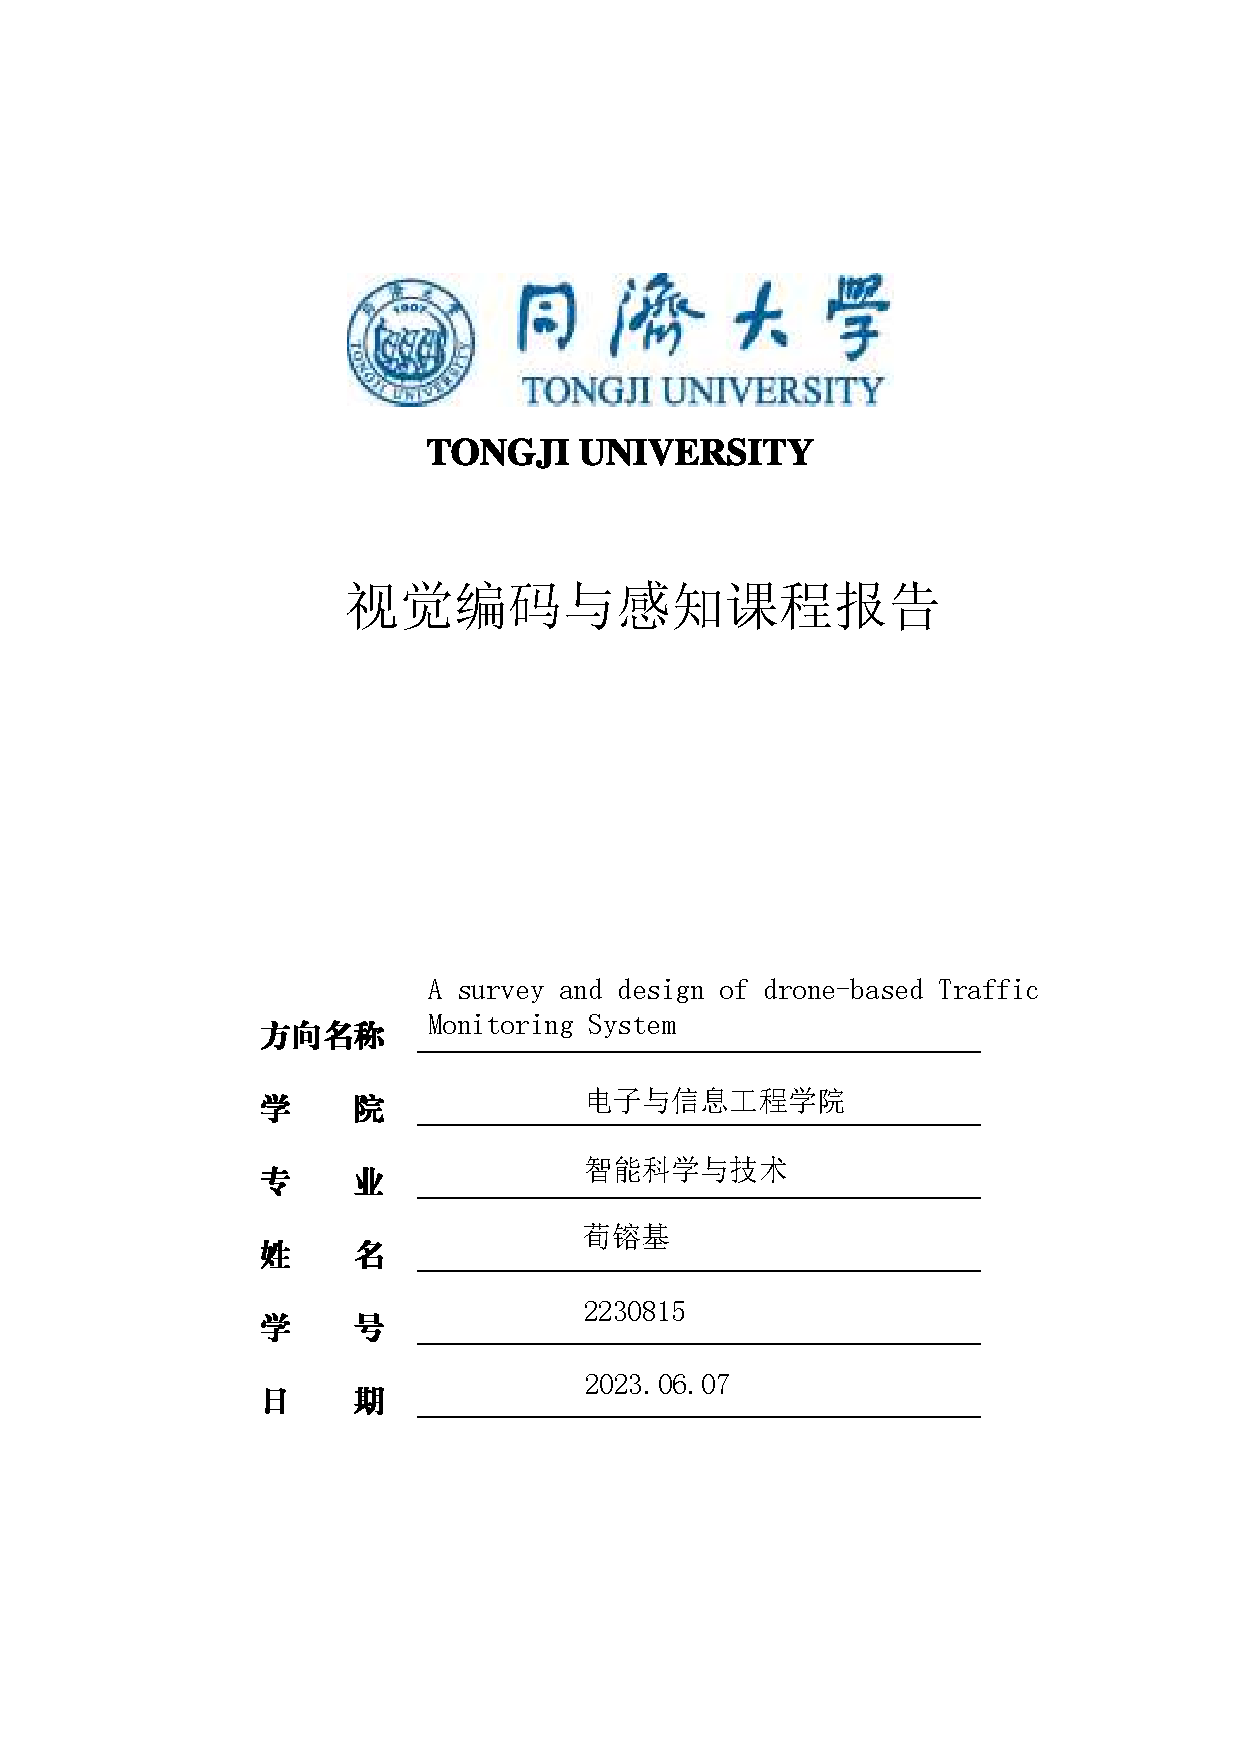
\includepdf[pages={1}]{./figures/视觉编码与感知报告封面.pdf} %曲线救国的思路,外界自建封面,然后调用
%\end{titlepage}

\date{}
%%%%%%%%% TITLE
\title{A survey and design of drone-based Traffic Monitoring System}

\author{Rongji Xun$^{1}$\\
	$^{1}$Tongji University\\
	{\tt\small 2230815@tongji.edu.cn, rongji.xun@gmail.com }
	\thanks{This is a course report for ``视频编码与视觉感知''}
	% For a paper whose authors are all at the same institution,
	% omit the following lines up until the closing ``}''.
% Additional authors and addresses can be added with ``\and'',
% just like the second author.
% To save space, use either the email address or home page, not both
}


% make the title area
\maketitle

%%%%%%%%% ABSTRACT
\begin{abstract}
	With the increasing constructions of city roads and highways, the surveillance ability provided by fixed-device on gantries becomes quite limited. In this case, drone-based monitoring system could boost the traffic surveillance ability in a more easy-deploying and location-flexible way. We firstly do some survey on current traffic monitoring systems. After that we arrange the related datasets, metrics and algorithms like MOT(multi object tracking), object detection methods. Most importantly, we present our design on traffic monitoring system and achieve quite a satisfying result on our collected video data. Our codes and models are available at \url{https://github.com/LokiXun/traffic_monitoring_system_survey_and_simple_design}
\end{abstract}


%%%%%%%%% BODY TEXT
\section{Introduction}
The continuous increase in number of motorized vehicles and the ever-increasing travel demands call for innovative and effective measures to be taken to tackle the challenges of high traffic volumes and congestion levels.\cite{khan2017uav} However, the existing infrastructure constrained by the fixed-device and location, could hardly cover all the scope in the city to have a general view of the city's traffic situation. For this purpose, deploying drones to monitor the traffic situation is a more flexible and efficient ways to solve the limited monitoring problems.

\begin{figure}[!t]
	\centering
	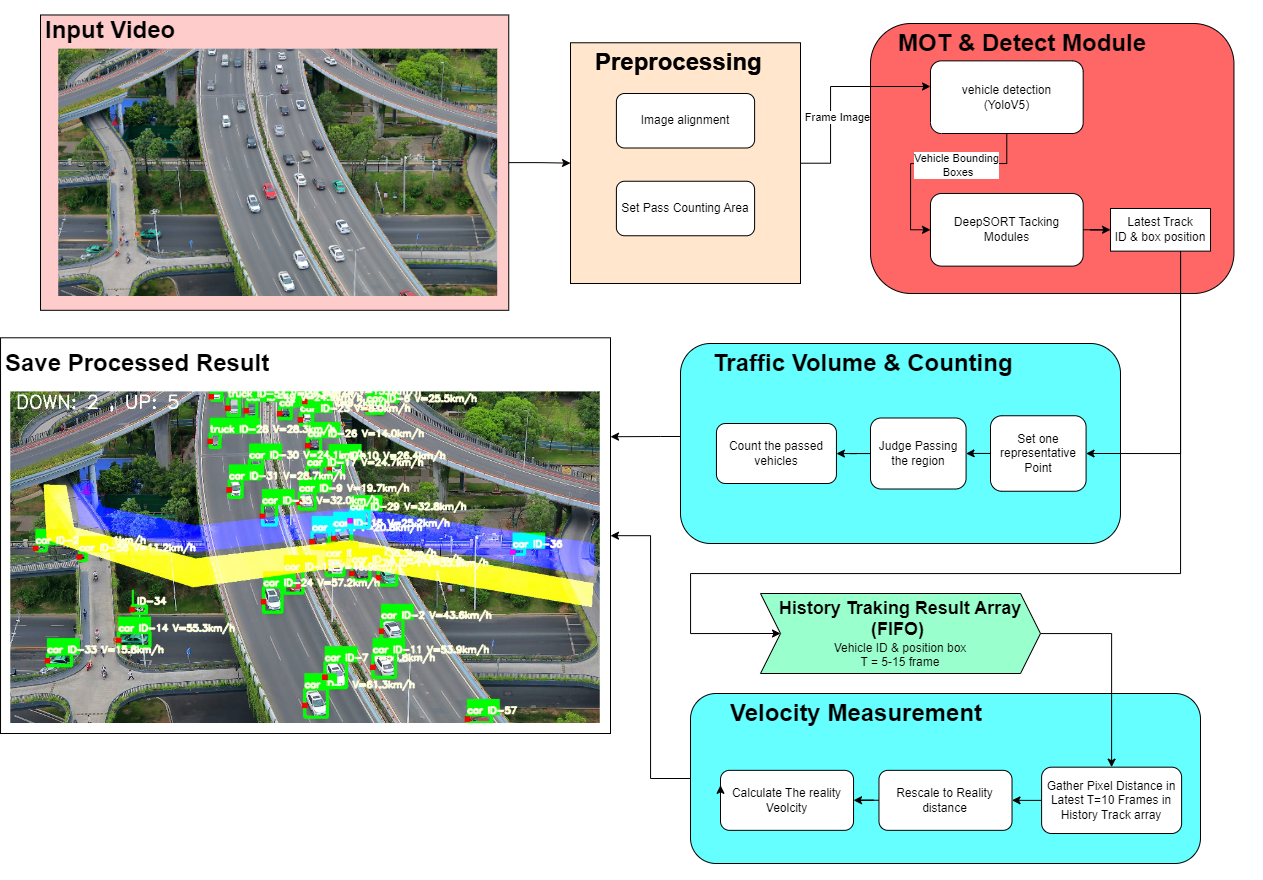
\includegraphics[width=0.95\linewidth]{./figures/traffic_monitoring_system_design.png} % requires the graphicx package
	\caption{Illustration of our Traffic Monitoring system framework. It incorporates MOT(Multi Object Tracking) methods to track cars in the video. The input videos are taken by drones and the drone could be steady in one position or moving with the object cars.}
	\label{fig:our-pipeline}
\end{figure}


There are some existing survey \cite{outay2020applications}, \cite{bisio2022systematic}, \cite{khan2017uav}, \cite{puri2005survey}, \cite{heintz2007images} of drone-based traffic monitoring system. Specially, \cite{bisio2022systematic} conduct a systematic review of drone-based traffic monitoring systems from a deep learning perspective. This work focuses on vehicle detection, tracking, and counting, since they are fundamental building blocks towards founding solutions for traffic congestion, flow rate and vehicle speed estimation. Additionally, drone-based datasets are examined, which face issues and problems caused by the diversity of features inherent of drone devices. The review analysis presented in \cite{bisio2022systematic} summarizes the literature solutions provided and deployed so far and discusses future research trends in establishing a comprehensive traffic monitoring system in support of the development of smart cities.

\cite{outay2020applications} presents a review of recent developments in relation to the application of UAVs in three major domains of transportation, namely; road safety, traffic monitoring and highway infrastructure management. Advances in computer vision algorithms to extract key features from UAV acquired videos and images are discussed along with the discussion on improvements made in traffic flow analysis methods, risk assessment and assistance in accident investigation and damage assessments for bridges and pavements. Additionally, barriers associated with the wide-scale deployment of UAVs technology are identified and countermeasures to overcome these barriers are discussed, along with their implications. 
\cite{puri2005survey} discusses and summarizes the research carried out all over the world until 2005 in the domain of UAV based traffic surveillance and analysis. \cite{heintz2007images} enlists and discusses the different modules of the proposed workflow i.e. flight planning, image acquisition and processing of UAV images. A particular focus is on the improvement of the UAV flight planning and control systems, eventually ensuring the quality of the acquired data. 


Unlike all existing surveys, we mainly focus on the overall framework of other drone-based monitoring system and also present our designed workflow by employing Deep learning based MOT(multi object Tracking) and object detection algorithms. To be more specific, as showed in Figure \ref{fig:our-pipeline}, we utilize YoloV5 \cite{github_yolov5} and DeepSORT \cite{wojke2017simple} in our project to detect and track the vehicles. The main contributions of this work are summarized as follows:
\begin{itemize}
	\item We categorize and summarize existing methods used in drone-based traffic monitoring system and make an in-depth and comprehensive survey on workflow design of drone-based traffic monitoring system. The summary provides insights for future algorithm design and new topic exploration.
	
	\item We summarize the widely used datasets and benchmark and analyze the approaches according to the object detection and tracking task in traffic monitoring system.
	
	\item We present our designed workflow illustrated in Figure \ref{fig:our-pipeline}, including vehicle velocity, volume and density measurement in traffic monitoring system.
\end{itemize}

The outline of this work is summarized as follows:
background and related works in traffic monitoring system are described in Sections \ref{section:related-work}. Sections \ref{section:methodology} to \ref{section:Datasets-metrics} covers some canonical object detection and MOT(multi object tracking) algorithms that related in traffic surveillance system. After that, in Section \ref{section:our-framework}, we illustrate our designed framework's principle and performance for three traffic monitoring tasks: volume,density,speed measurement. Eventually, in Section \ref{section:conclusion} the conclusions are drawn.

%\tableofcontents
%\newpage




\section{Related Works}
\label{section:related-work}
In this section, we would discuss the related survey and works about traffic monitoring systems. \cite{jian2019combining} designs a general drone-based traffic congestion recognition workflow illustrated in Figure \ref{fig:jian2019combining_workflow}: images/videos acquisition, data processing and using CNN to make recognition result and send back to Traffic-Management Center.
\cite{khan2017uav} presents a detailed guide on implementing a UAV-based traffic monitoring system showed in Figure \ref{fig:khan2017uav_workflow}: firstly define the scope (decide the project objective, select the monitoring region like ramp or roadway segment and measure performance which is varied with the task like traffic volume, vehicle velocities). Then do the flight planning and dispatch the drones to take videos/images data. Finally analysis the data and optimize for defined task. In these schemes, the analyzing part in drone-based monitoring tasks can be done either on-board or via cloud-based processing.

\begin{figure}[!t]
	\centering
	\subfigure{\begin{minipage}[t]{1\linewidth}
		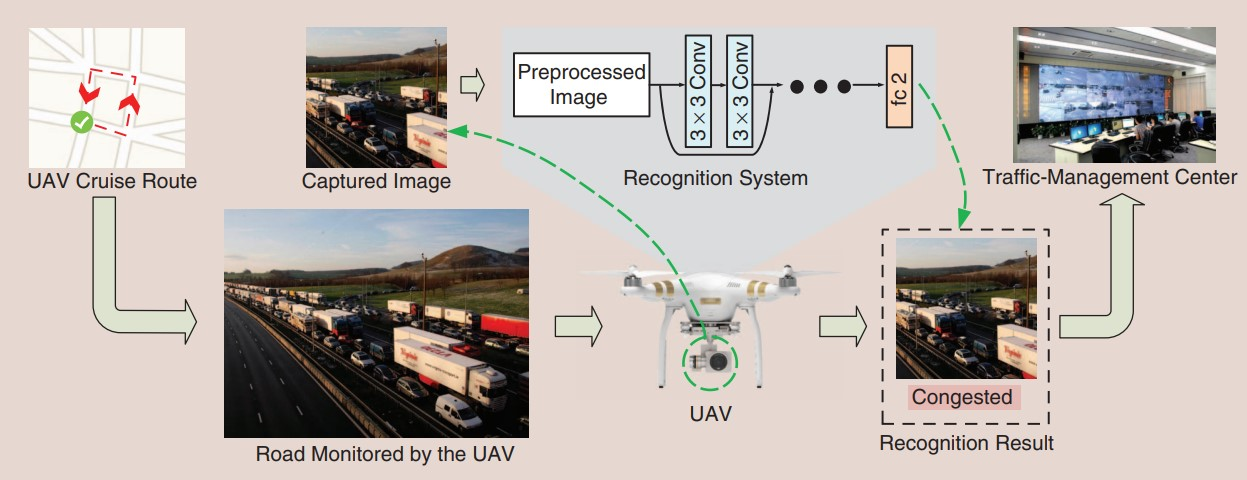
\includegraphics[width=0.95\linewidth]{./figures/Framework_in_Combining unmanned aerial vehicles with artificial-intelligence technology for traffic-congestion recognition.jpg} % requires the graphicx package
		\caption{A schematic used in \cite{jian2019combining} illustrating how a UAV-based traffic-congestion monitoring system works}
		\label{fig:jian2019combining_workflow}
	\end{minipage}}

	\subfigure{\begin{minipage}[t]{1\linewidth}
			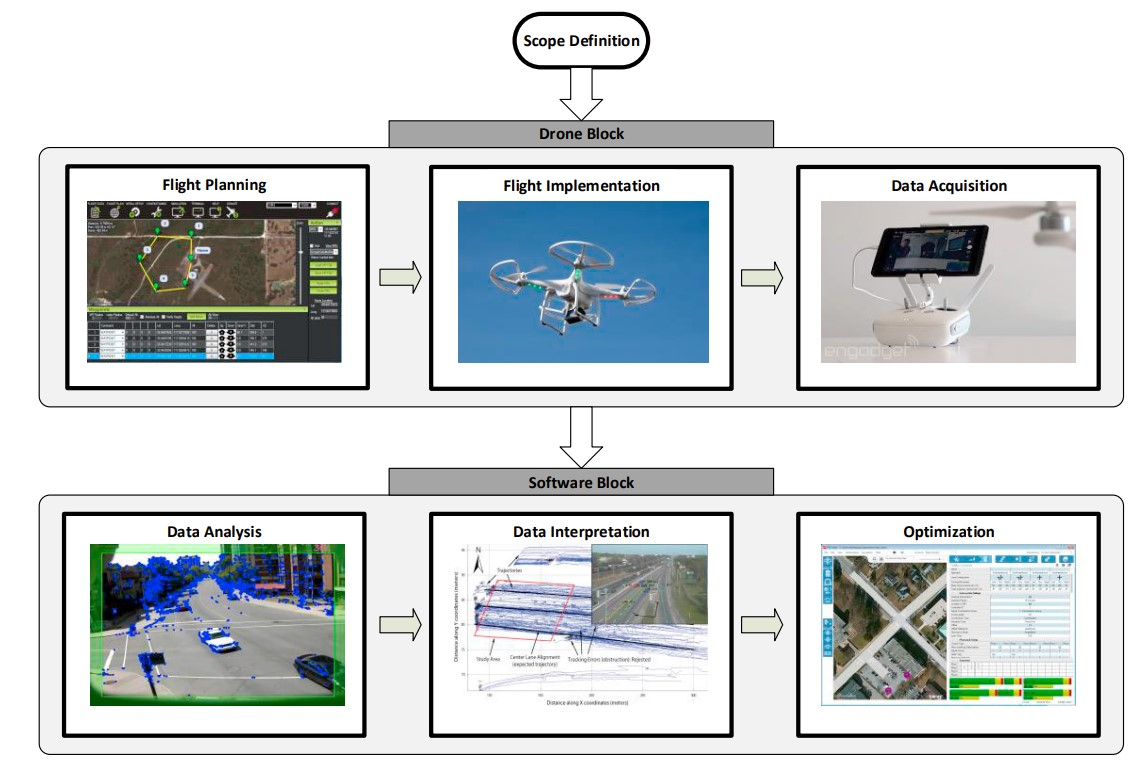
\includegraphics[width=0.95\linewidth]{./figures/khan2017uav_pipline.jpg} % requires the graphicx package
			\caption{A detailed workflow used by \cite{khan2017uav}, including scope definition, route planing, data processing part.}
			\label{fig:khan2017uav_workflow}
	\end{minipage}}
	\centering
	
\end{figure}

As discussed above, implementing drone-based traffic monitoring tasks in urban areas and on highways is quite challenging due to the multitude of challenges in the acquired videos and images. This ultimately makes it more difficult to attain the highest level of accuracy for various traffic monitoring tasks (vehicle identification, tracking, counting, and speed estimation, for example) \cite{bisio2022systematic}.

For the vehicle detection methods could be roughly split into two categories: 1) background segmentation: \cite{zhou2007moving} firstly divide image into small non-overlapped blocks and send the extracted PCA feature to SVM classifier judging whether the blocks belongs to any vehicle.  \cite{xu2016background} also employed a background subtraction technique and tested to be valid on various kind of scenes. 2) feature extraction based detection. Different object features, like Scale Invariant Feature Transformation (SIFT) used in \cite{mu2016multiple}, Haar-like features used in \cite{han2009vehicle}, and Histogram of oriented Gradients (HoG) are utilized in \cite{dalal2005histograms} to detect humans. 

In comparison, with the performance of Deep Learning methods soaring, some Deep Learning based works like \cite{li2019simultaneously}, \cite{zhu2018urban}, \cite{micheal2019automatic} are widely adopted.
% DL methods in traffic monitoring ---------------------
\cite{li2019simultaneously} introduced a novel method for simultaneously detecting and counting vehicles in drone-based scenes, illustrated in Figure \ref{fig:li2019simultaneously_framework}. This task was challenging because the targets are small and dense. The authors analyzed the reasons behind this problem, including how to select the suitable anchor boxes and how to extract the features of small objects. Then, they proposed an SA strategy to select anchors and apply circular flow to guide feature extraction. In addition, they proposed adding the counting regularized constraint to the object detection task for further improving performance. \cite{dong2015vehicle} propose a vehicle type classification method using a semi-supervised convolutional neural network from vehicle frontal-view images and introduce sparse Laplacian filter learning to obtain the filters of network with large amounts of unlabeled data. 

The difference between static and video object detection frameworks lies in the incorporation of temporal information. Furthermore, although video object detection and Multi-Object Tracking (MOT) both use UAV video data, the way temporal information is employed differs in the two cases. The former aims at improving the detection rate of the current frame by exploiting context information from previous frames, while the latter aims at forecasting the trajectory of objects in future frames. Furthermore, in UAV-based videos the movements of the camera within a scene, usually referred to as ego motion, complicate vehicle detection and other traffic monitoring tasks significantly. Prior to the advent of DL-based frameworks, this issue was addressed in two distinct ways \cite{bisio2022systematic}: image registration \cite{yalcin2005flow},\cite{angel2003methods},\cite{cao2012vehicle} and optical flow \cite{cao2012vehicle} \cite{yalcin2005flow}, \cite{ke2016real}. \cite{angel2003methods} proposed an approach for collecting and analyzing aerial imagery is given. To illustrate the value of the imagery, the paper outlines methods to generate estimates of speeds, travel times, densities, and queueing delays. In \cite{cao2012vehicle}, to solve the problems like UAV motion, scene complexity, and especially the partial occlusion of targets, multi-motion layer analysis methods is proposed to detect and track moving vehicles in airborne platform. 

In image registration solutions, moving background is turned into a fixed one, hence facilitating the background subtraction task \cite{zhou2007moving} to overcome the ego motion issue. On the other hand, optical flow combined with supervised learning enables the detection of vehicles in a dense traffic environment using a UAV video with ego motion \cite{bisio2022systematic}.


\begin{figure}[!t]
	\centering
	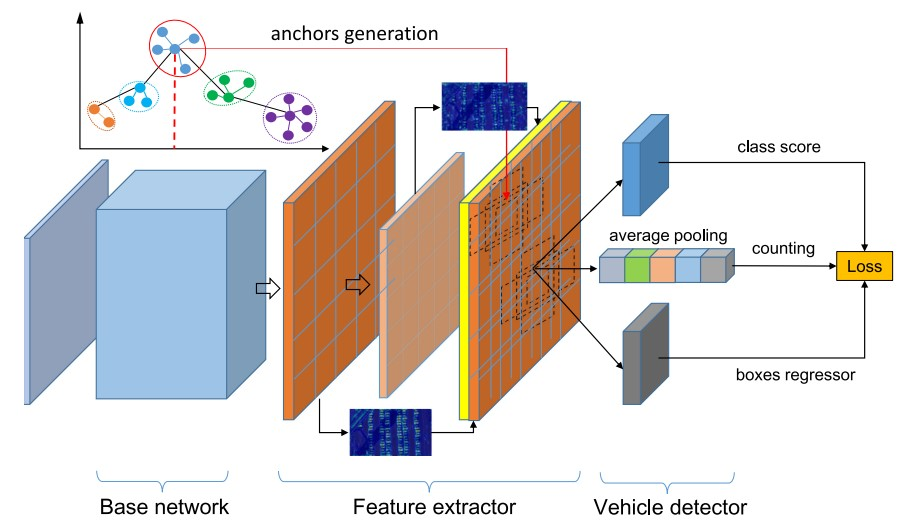
\includegraphics[width=0.95\linewidth]{./figures/li2019simultaneously_framework.jpg} % requires the graphicx package
	\caption{Overview of \cite{li2019simultaneously}'s approach. propose a unified full CNN to localize and count vehicles in the drone-based images. It consists of three parts: a base network, a feature extractor, and a vehicle detector. They introduce an SA strategy to generate the suitable anchor boxes. A circular flow is embedded in the feature extractor by combining the bottom-up cues with top-down attention. And they build the counting layer and introduce a counting regularized term into the original loss.}
	\label{fig:li2019simultaneously_framework}
\end{figure}

 

\section{Methodology}
\label{section:methodology}
\subsection{Traffic Object Detection}
In drone-based traffic monitoring system, the images taken by drones may suffer from occlusion, varying size and orientation, so that directly training the vehicle detector on ImageNet \cite{russakovsky2015imagenet} and \cite{lin2014microsoft} datasets is hard to produce high performance. \cite{le2018combining} proposed a vehicle classification system for drone imagery that combines transfer learning features from the Inception-ResNet v2 model with hand-made features \cite{szegedy2017inception}. \cite{li2020multi} proposed Scale-Specific Prediction-Single Shot MultiBox Detector (SSP-SSD) framework to solve the multi-scale issue in aerial images. 
However, most traffic surveillance datasets only contain the day time images and the deficit of night time data may harm the generalization ability of the detectors. \cite{li2021domain} proposed a framework using Faster R-CNN \cite{ren2015faster}, with domain adaptation for detection and using cycle GAN approach \cite{zhu2017unpaired} to turn daytime data into unlabeled night ones. 

For video-based Detection methods, a shortlisted studies on drone-based video monitoring system are summarized in Table \ref{table:video-detector result}. \cite{biswas2019speed} choose Faster R-CNN \cite{ren2015faster}, illustrated in Figure \ref{fig:biswas2019speed_FasterRCNN_workflow}, to detect the small and large vehicles.

\begin{table*}[!t]
	\centering
	\resizebox{\textwidth}{!}{
	\begin{tabular}{ccccccccccc}
		\hline
		Framework & Backbone Model & Dataset(s) & Image Resolution & Altitude & UAV/Camera state & Object class & \multicolumn{4}{c}{Outcome} \\
		\cline{8-11}
		\centering ~ & ~ & ~ & ~ & ~ & ~ & ~ & AP/mAP(\%) & F1/mF1(\%) & Accuracy(\%) & Quality(\%) \\
		\hline
		Enhanced SSD & ResNet-101 & UAVct & 3840$\times$2178(30fps) & 126m	& Mostly top view & 3(Cars,Bus \& Truck) & -- & -- & -- & 86.4\\
		Faster R-CNN & VGG-16 &  \makecell{i.UAV123 \\ ii.VIVID} & \makecell{i.1280 $\times$  720 \\ ii.640 $\times$ 480} & \makecell{i.5m\\ ii.High altitude} & Different views & 1(Cars) & \makecell{i.96.03 \\ ii.96.19} & -- & -- & --\\
		YOLOv3 & Darknet-53 & \makecell{Custom + aerial cars \\datasets \cite{adaimi2020perceiving} + \\UAVDT }& $2720 \times 1530$(30fps) & Different altitudes & Different angles & -- & -- & 92.10 & -- & -- \\
		YOLO & CNN & Custom & -- & -- & -- & 2(Car \& Bus) & -- & -- & 84 & --\\
		\hline
	\end{tabular}
	}
	\caption{Summary and comparison of DL-based vehicle detection systems using drone video data \cite{bisio2022systematic}}
	\vspace{-10pt}
	\label{table:video-detector result}
\end{table*}

\begin{figure}[!t]
	\centering
	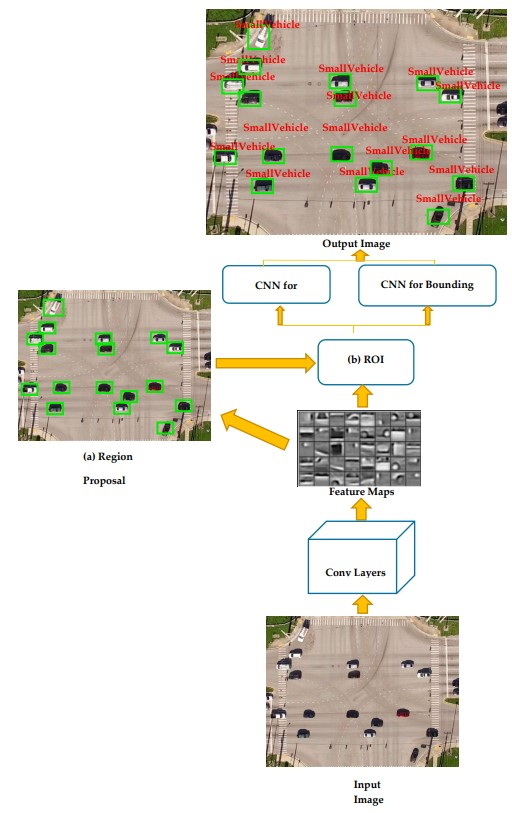
\includegraphics[width=0.95\linewidth]{./figures/biswas2019speed_FasterRCNN_workflow.jpg} % requires the graphicx package
	\caption{Faster region-based convolutional neural network (R-CNN) architecture used in \cite{biswas2019speed}}
	\label{fig:biswas2019speed_FasterRCNN_workflow}
\end{figure}

\subsection{Multi Object Tracking}
In a broader view, tracking algorithms can be classified as online/offline, SOT/MOT(Single/Multi Object Tracking), and detection-based/detection-free. In SOT approaches, objects are tracked through their entire motion, independently of their detection, whereas in MOT methods, objects are tracked only if they are first detected and localized. Furthermore, MOT solutions employ both offline and online approaches, where offline methods achieve better performance, while online solutions prove more robust. 

Various approaches to object tracking have been proposed in the literature, such as Intersection over Union (IoU)-based tracking \cite{yu2022frequency}, Simple Online and Real-Time Tracking(SORT)\cite{bewley2016simple}, DeepSORT \cite{wojke2017simple}. And Figure \ref{fig:bewley2016simple_SORT_framework_SORT} illustrated the workflow of SORT \cite{bewley2016simple}.
In comparison to this, SORT \cite{bewley2016simple}, an online algorithm, showed higher precision and accuracy, although it is also vulnerable to certain false positives, and this deficiency is tackled by the DeepSORT algorithm \cite{wojke2017simple}. Other widely employed techniques available in the literature to the purpose of objects tracking are particle filtering, Discriminative Correlation Filter (DCF), Kalman Filtering (KF) \cite{cuevas2005kalman}, \cite{chui2017kalman}.


\begin{figure}[!t]
	\centering
	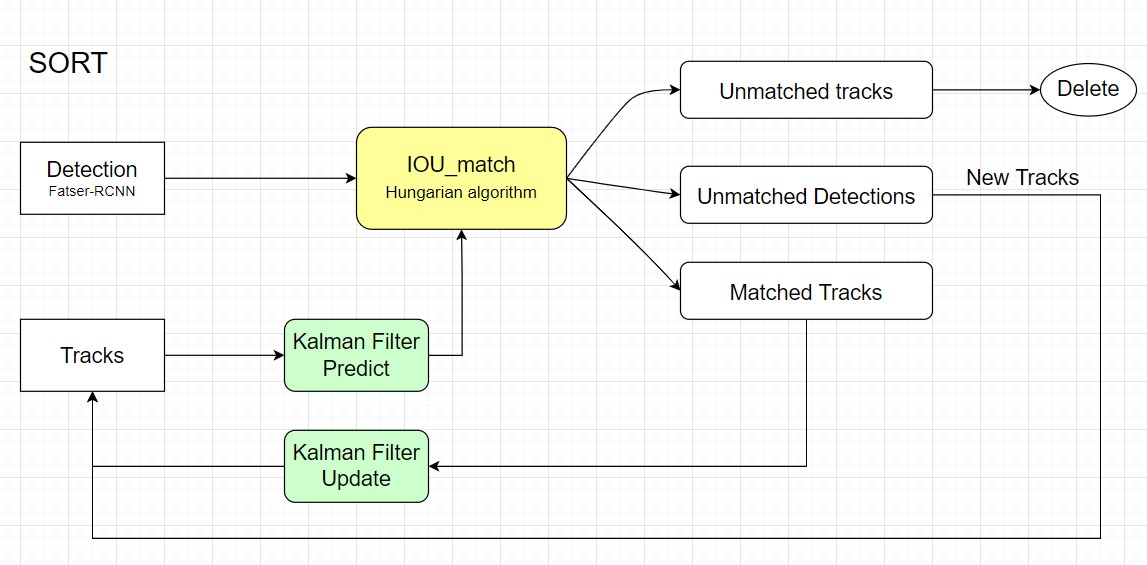
\includegraphics[width=0.95\linewidth]{./figures/MOT_framework_SORT.jpg} % requires the graphicx package
	\caption{SORT \cite{bewley2016simple} overall workflow}
	\label{fig:bewley2016simple_SORT_framework_SORT}
\end{figure}




\section{Traffic Datasets And Evaluating Metrics}
\label{section:Datasets-metrics}
\subsection{Dataset}
Different from traditional image classification task, the traffics images that the drones acquired would have various shooting angles, high-density vehicles and tiny target size. These all resort to drones' shooting environment: 1)  wide angle camera make images contains high density vehicles; 2) moving drones and target objects contribute to image rotation, blurring problem; 3) tiny target size due to the high altitude.

To address the above issues, the availability of appropriate
datasets is a fundamental step towards finding suitable algorithmic solutions. In this connection, Convolutional Neural Networks (CNNs) are typically employed for image processing, and they are data hungry \cite{waqas2019isaid}.

In recent years, researchers have produced various drone-based aerial datasets to address data availability issues for different applications, which boost the development of drone-based vehicles detection and Tracking methods.\cite{bisio2022systematic}

The dataset presented in \cite{mueller2016benchmark} contains 110k frames to the purpose of object tracking from an aerial view. This dataset has been 285
acquired at low UAV altitude, with moving camera, and 286
different shooting angles, due to UAV motion \cite{bisio2022systematic}. Though \cite{mueller2016benchmark} lacks the data for dynamic weather and altitude settings, the moving camera and other features make it suitable for traffic monitoring task.

Visdrone \cite{zhu2021detection}, \cite{zhu2018vision}, the largest drone-based aerial datasets, which could be applied to four tasks: object detection in images or videos, object tracking like SOT and MOT. It includes 263 video sequences and more than 10000 static images, all of which were collected using various drones in 14 different cities in diverse weather and lighting conditions and 301
at various altitudes \cite{bisio2022systematic}.

Also, UAV Detection and Tracking (UAVDT) \cite{du2018unmanned} contains 80k images/Frames, with 1080$\times$540  resolutions, taken in 10-70m altitude with multiple camera-view. Mostly it is used for SOT(single object tracking) task. \cite{jensen2020presenting} proposed in 2020, an aerial dataset of a road scene is produced a static and a drone based camera, contains 4 object classes and 3.1k images in 1920$\times$ 1080 resolution and mainly used for traffic object detection task. Furthermore, Stanford Drone \cite{robicquet2016learning} includes six categories for objects. And the bicyclists, car and bus targets could be used for traffic surveillance task. 

\subsection{Object Detection Metrics}
To assess the performance of object detection, precision, recall and Average Precision (AP), followed by the detection speed are the most widely used metrics. Usually binary predictions results are accessed with respect to the Ground Truth (GT) as True Positive (TP), True Negative (TN), False Positive (FP) and False Negative (FN). However, Detectors usually generates lots of Bounding Boxes (BBoxes) that are not required to be predicted. So that TN is usually not used for accessing detector's performance \cite{padilla2020survey}.
The evaluating metrics, precision and recall, of the object detection algorithm are defined as follows:

\begin{equation}
	\label{eq:PR_metrics}
\begin{aligned}
	&Precision = \frac{TP}{TP+FP} \\
	&Recall = \frac{TP}{TP+FN}
\end{aligned}
\end{equation}


Given in \cite{du2018unmanned}, since precision and recall metrics do not include TN prediction, the Precision-Recall (PR)-curve is also employed as an evaluating metric to examine the performance of the detector, particularly for the unbalanced datasets. An optimal detector's PR curve should have high AP, which refer to  Area Under the Precision-Recall Curve(AUC-PR). The zig-zag pattern in PR curve may cause difficult to calculate the AP value. So that 11-point or all-point interpolation methods is used in \cite{everingham2015pascal}, which may decrease the AP value. Increasing the IoU threshold, on the other hand, decreases the AP value, and vice versa. For multi-class situation, predictions are made separately for each category, and the mean AP (mAP) metric is used to assess the overall performance of object detectors \cite{bisio2022systematic}.
\begin{equation}
	\label{eq:mAP_metrics}
\begin{aligned}
	&mAP = \frac{1}{m} \sum_{j=1}^{m} AP_j \\
	&where~m~denotes~class~number.
\end{aligned}
\end{equation}


\subsection{Object Tracking Metrics}
Some canonical object tracker \cite{bewley2016simple}, \cite{wojke2017simple} have been evaluated using the following metrics, which are summarized in \cite{bisio2022systematic}:
\begin{itemize}
	\item Recall: It indicates ratio of correctly matched objects among all GT objects.
	\item Precision: It measures the ratio of correctly matched objects among all output objects.
	\item False Alarms: The number of FAs/frame.
	\item FP: The number of false positives or false detections.
	\item FN: The number of FN/frame or missed detections.
	\item GT: The number of GT trajectories.
	\item Mostly Tracked (MT): The number of target trajectories covered by tracker for more than or at least 80\% of the trajectory length.
	\item Mostly Lost (ML): The number of target trajectories covered by tracker for less than or at least 20\% of the trajectory length.
	\item Fragments (Frag): The number of times a tracked trajectory is interrupted.
	\item IDentity Switches (IDS): The number of times an object ID changes to another ID.
	\item MOTA(MOT Accuracy): is the main metric in MOT(multi object tracking) to access the tracking ability and not considering the detection accuracy. illustrated in Equation \ref{eq:MOTA_MOTP}.
	\item MOTP:(MOT Precision): reflects the average dissimilarity between the obtained true positives and corresponding GT targets. illustrated in Equation \ref{eq:MOTA_MOTP}.
	
\end{itemize}
\begin{equation}
	\label{eq:MOTA_MOTP}
	\begin{aligned}
		&MOTA = 1 - \frac{\sum_t(FN_t + FP_t + IDSW_t)}{\sum_t GT_t}\\
		&MOTP = \frac{\sum_{t,i} d_{t,i}}{\sum_t{c_t}} \\
	\end{aligned}
\end{equation}

In an optimal tracker, precision, recall, MT, and GT metrics should provide high values, whereas FA, FN, FP, ML, Frag, and IDS indicators should be low. MOTA and MOTP values should be higher for an efficient and accurate tracker. MOTA and MOTP are illustrated in Equation \ref{eq:MOTA_MOTP}, where $FN_t$ is False Negative, $FP$ is False Positive, $IDSW$ is ID Switch, $GT$ is Ground Truth object Number. $d_{ij}$ is the distance between predicted and ground truth position, which usually using the overlap rate.


\section{Our System Framework}
\label{section:our-framework}
\subsection{Our design}
Figure \ref{fig:our-pipeline} illustrates our Traffic Monitoring system framework. We choose YoloV5 \cite{github_yolov5} and DeepSORT \cite{wojke2017simple} as our detector and tracker. Our workflow contains the following modules: input video preprocessing module, Tracking \& Detection block and 3 task specific modules: vehicle volume, density and velocity measurement module.


More specifically, the input video frame may have various resolution and different from the detector's input size. For preprocessing module, we simply down-sample the input image to $960 \times 540$ resolution, according with the detector network's input size and decreasing the computation complexity to speed up the inference process. Furthermore, we assume that the input video may not suffer from large mismatch and in later version add some image alignment methods to eliminate this assumption.

Then is the Tracking module, firstly the detector YOLOv5 \cite{github_yolov5} detect the vehicles in current frame and send the detection bounding boxes as inputs to the DeepSORT. And tracker use current detection result and previous track to update the new track and Re-ID the vehicles. SO at this time we have already got current frame's tracking result, which contains vehicles' ID, bounding box position, class label and confidence. These track data would serve as the input for later task specific modules, which are velocity, volume, density measurement module.

\begin{figure}[htbp]
	\centering
	\subfigure[original input frame]{
		\begin{minipage}[t]{0.33\linewidth}
			\centering
			\includegraphics[width=1in]{./figures/demo_original_frame.png}
			\label{fig:our-tracking-result-a}
		\end{minipage}%
	}%
	\subfigure[add Volume region]{
		\begin{minipage}[t]{0.33\linewidth}
			\centering
			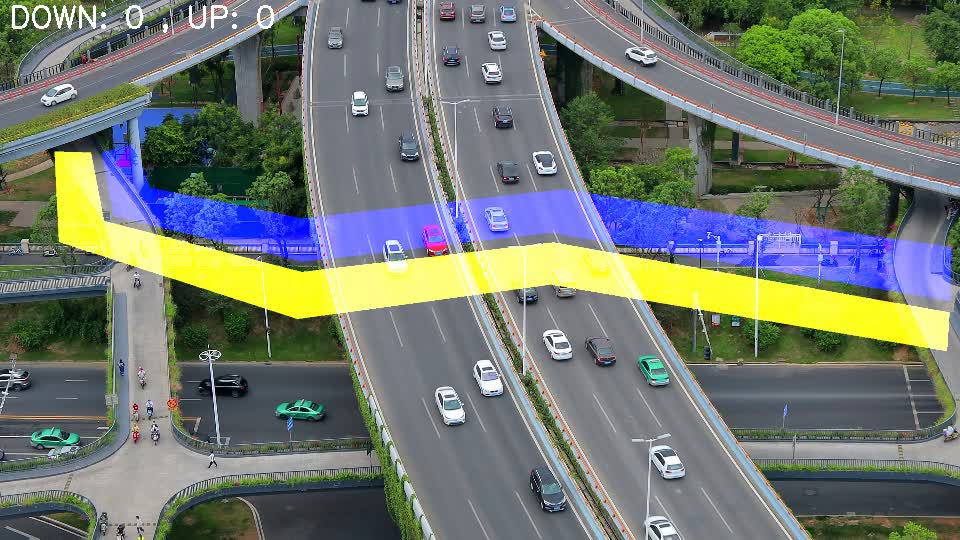
\includegraphics[width=1in]{./figures/demo_count_region.png}
			\label{fig:our-tracking-result-b}
		\end{minipage}%
	}%
	\subfigure[overall processed result]{
		\begin{minipage}[t]{0.33\linewidth}
			\centering
			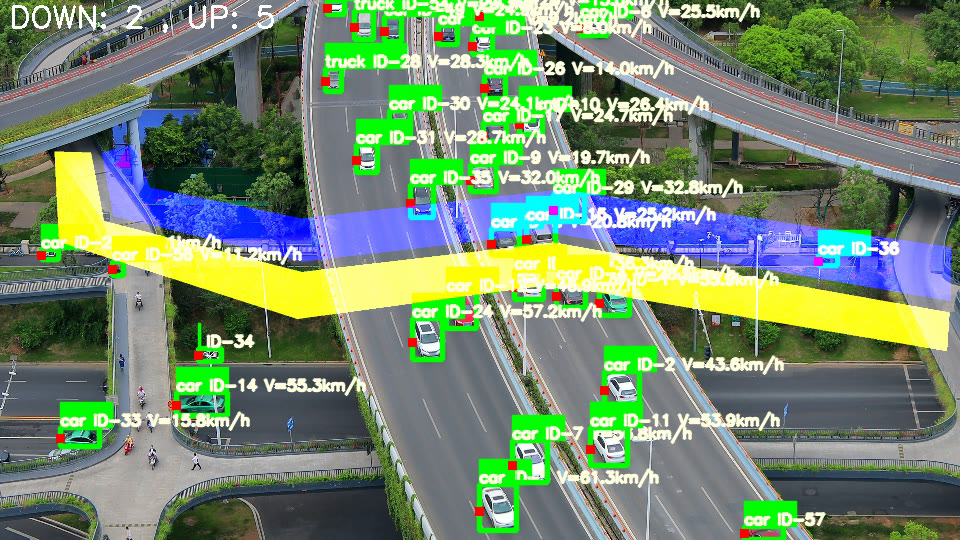
\includegraphics[width=1in]{./figures/demo_process_result.png}\\
			\label{fig:our-tracking-result-c}
		\end{minipage}
	}%
	\centering
	\vspace{0.2cm}
	\caption{The Tracking Result for one frame in video.}
	\label{fig:our-tracking-result}
\end{figure}

\subsection{Traffic Volume}
Constrained by the drones' limited view and the dynamic moving of vehicles, we assume to put drone be settled in the one place to overlook the road. In this setting, we count the numbers of vehicles that pass through the designated region to calculate the traffic volume for a period. 

The passing region's multi-polygon in our experiment is assign by hand-made positions. As illustrated in Figure \ref{fig:our-tracking-result-b}, we set 2 regions to denote the act of entry and exit. We consider a vehicle passed when the car firstly passes through the enter region, then into the exit region and finally leave the exit region. For the realization, we just create 2 ID sets for entry and exit region to check the vehicle status for entry or exit.


\subsection{Traffic Density}
Probably the most straight-forward traffic application of aerial images is the determination of density (in vehicle/km/lane) because it provides snapshots of segments of roadway at one instant in time. The basic estimate of density can be obtained by manually counting the number of vehicles in an image and dividing it by the field of view of the image and the number of lanes. As a matter of fact, a few companies currently use this method commercially to conduct congestion studies \cite{angel2003methods}.

For the Traffic Density, we simply follow \cite{angel2003methods} to calculate the number of vehicles had been detected in the current frame and divided by the view's area.



\subsection{Vehicle Velocity}

\cite{biswas2019speed}, their workflow illustrated in Figure \ref{fig:biswas2019speed_complete_framework}, consider both static and moving states of UAV while recording video with optical camera. For detector, the author choose Faster R-CNN \cite{ren2015faster} to detect the small and large vehicles. For tracker, the autor choose CSRT \cite{lunevzivc2018discriminative}, which uses a spatial reliability map to adjust filter support to the part of selected region from the frame for tracking. Since a moving platform of a drone would causing view's motion, they also incorporate Feature-Based Image Alignment (FBIA) technique and Structural Similarity Index Measurement (SSIM) to preprocess the frame coherence to ensure the traking performance. Specifically, FBIA was employed on each frame to ensure the true object location while the SSIM metrics was used to measure the similarity between consecutive frames.

To measure the velocity, the traveled distance of a vehicle is calculated by measuring the centroid displacement of the vehicle from the reference frame to the current frame. Finally, vehicles' speed is measured by the traveled distance with respect to time (traveling time is calculated from the frame rate) \cite{biswas2019speed}. 

\begin{equation}
	\label{eq:velocity-equation}
	\begin{aligned}
		VelocityActual = \frac{PixelDistance * Pixel2RealityScale}{FrameNum * 1/FPS}
	\end{aligned}
\end{equation}

In our project, we follow \cite{biswas2019speed} way and using a FIFO(first in first out) array to store the history track positions of identified vehicles. Note that: 1) the element in array is the track info, which contains the vehicles' ID and  bounding boxes position; 2) the history frames number we consider here is 10 frames. Specifically, measuring the velocity for a specific vehicle, we take its ID to get the history frames, accumulate the pixel-distance in history tracks and divide the distance by time duration for $T=10$ frames with Equation \ref{eq:velocity-equation}. For the scale value mapping the pixel distance to reality, we simply assume that the car is 5 meters long and get the car's object bounding box length to calculate the actual distance for each pixel length.


\begin{figure}[!t]
	\centering
	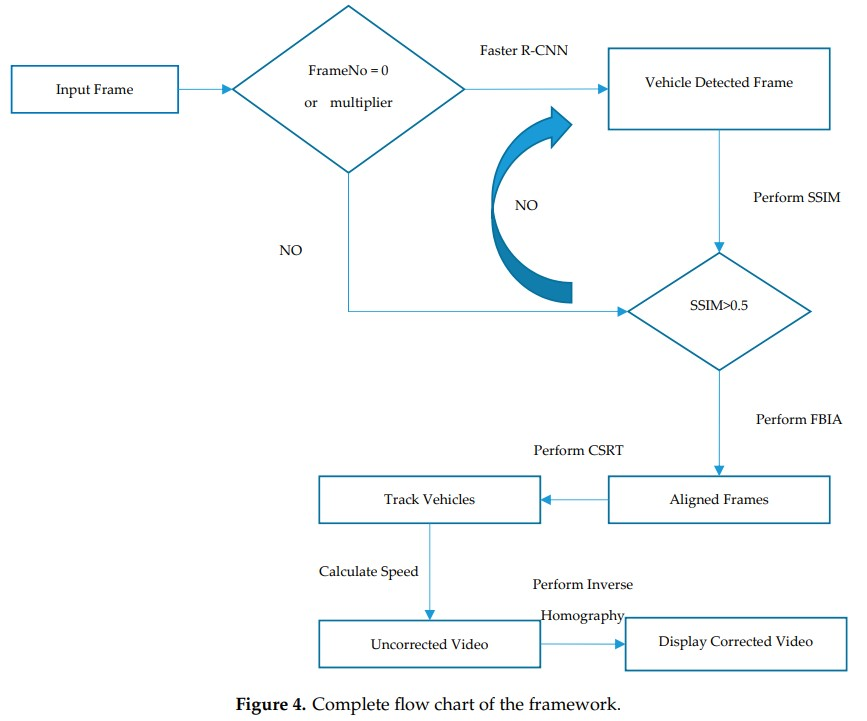
\includegraphics[width=0.95\linewidth]{./figures/biswas2019speed_complete_framework.jpg} % requires the graphicx package
	\caption{the complete workflow in \cite{biswas2019speed}}
	\label{fig:biswas2019speed_complete_framework}
\end{figure}


\subsection{Experiment and limitations}
Figure \ref{fig:our-tracking-result} shows our tracking result for one video taken by drones. We are able to accurately track most of the vehicles, count the traffic volumes and velocity for each vehicle. However, the speed may not be that accurate because drone's view is not absolute parallel with the ground and there exists a vanishing point effect, which means the pixel distance in further point of image is relative larger in the reality. And this error in pixel distance may harm the distances we added in the history frame and eventually make the measurement not that precise. At the same time, there is still some vehicles with tiny size in image are not able to be detected by detectors.

In the future, calculating the vehicles' track to get the distance and improving the detecting ability for the tiny size objects are good directions for improvement.


\section{Conclusion}
\label{section:conclusion}
In this work, we firstly summarize existing systems for drone-based traffic monitoring. And we illustrate several canonical datasets and methods in Object Tracking and Detection field. Also we present our framework, using YoloV5 detector and DeepSORT tracker is applied to detect and track the vehicle in videos, and achieve an acceptable performance for measuring the traffic volume, density and speed. However, there  the detector's performance for detecting vehicles is still not that ideal for tiny size vehicles. 

\section*{Acknowledgment}
During this process of doing survey on related systems' paper, we learn lots of MOT, Object detection algorithms which might be helpful in our future research.


% references section
{\small
	\bibliographystyle{ieee_fullname}
	\bibliography{egbib}
}

\end{document}

